\documentclass[tikz,border=6pt]{standalone}
\usepackage{xcolor}
\usetikzlibrary{decorations.pathmorphing} % for squiggly arrows
\begin{document}
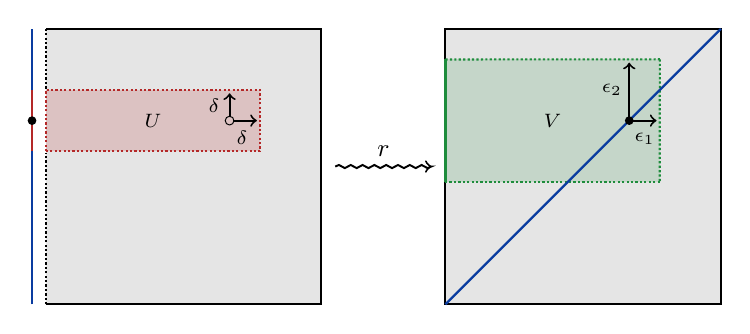
\begin{tikzpicture}[scale=3.5]
  % Colors
  \definecolor{myblue}{RGB}{10,60,160} % strong dark blue
  \definecolor{mygreen}{RGB}{30,140,60}
  \definecolor{myred}{RGB}{180,40,40}

  % Parameters (use \offset so \delta remains the Greek letter for labels)
  \def\offset{0.05}   % left square offset
  \def\shiftTwo{1.5}  % second square left edge

  % dot / circle sizes (very small)
  \def\dr{0.45pt}   % dot radius
  \def\crad{0.45pt}  % circle radius (slightly bigger than dot)
  \def\shorten{1.2pt} % arrow shorten amount to avoid overlapping dot

  % --- Diagram 1 ---
  % Thick blue vertical line from (0,0) to (0,1) with arrow up
  \draw[line width=0.8pt, myblue] (0,0) -- (0,1);

  % Light gray filled square shifted right by offset
  \fill[gray!20] (\offset,0) rectangle ({1+\offset},1);

  % Square outline, left side dashed
  \draw[line width=0.7pt] (\offset,0) -- ({1+\offset},0) -- ({1+\offset},1) -- (\offset,1);
  \draw[line width=0.7pt, dash pattern=on 0.8pt off 0.8pt] (\offset,0) -- (\offset, {5/9-0.005});
  \draw[line width=0.7pt, dash pattern=on 0.8pt off 0.8pt] (\offset,1) -- (\offset, {7/9+0.005});

  % --- Red sub-rectangle inside first square (unchanged dims) ---
  \coordinate (rll) at ({\offset+0}, {5/9});
  \coordinate (rur) at ({\offset+7/9}, {7/9});
  \fill[myred, opacity=0.18] (rll) rectangle (rur);
  \draw[line width=0.8pt, myred, dash pattern=on 0.8pt off 0.8pt] (rll) rectangle (rur);

  % Separate solid red line placed on the blue axis x=0 (independent)
  \draw[line width=0.9pt, myred] (0,{5/9}) -- (0,{7/9});

  % label for red region
  \node[font=\scriptsize] at ({\offset + 7/18}, {2/3}) {$U$};

  % small unfilled circle at (offset + 2/3, 2/3) inside left square (thin outline)
  \coordinate (leftCircleCenter) at ({\offset + 2/3}, {2/3});
  \draw[line width=0.35pt] (leftCircleCenter) circle (\crad);

  % --- Squiggly arrow with "r" between diagrams ---
  \coordinate (start) at ({1+\offset + 0.05},0.5);
  \coordinate (end)   at ({1+\offset + 0.4},0.5);
  \draw[->, decorate, decoration={snake, amplitude=0.2mm, segment length=1.5mm}, line width=0.7pt]
    (start) -- node[above,font=\small] {$r$} (end);

  % --- Diagram 2 ---
  \fill[gray!20] (\shiftTwo,0) rectangle ({1+\shiftTwo},1);
  \draw[line width=0.7pt] (\shiftTwo,0) -- ({1+\shiftTwo},0) -- ({1+\shiftTwo},1) -- (\shiftTwo,1) -- cycle;
  \draw[line width=0.7pt, dash pattern=on 0.8pt off 0.8pt] (\shiftTwo,0) -- (\shiftTwo,1);

  % --- Green sub-rectangle inside second square (unchanged) ---
  \coordinate (G_ll) at ({\shiftTwo+0}, {4/9});
  \coordinate (G_ur) at ({\shiftTwo+7/9}, {8/9});
  \fill[mygreen, opacity=0.16] (G_ll) rectangle (G_ur);
  \draw[line width=0.9pt, mygreen] ({\shiftTwo},{4/9}) -- ({\shiftTwo},{8/9});
  \draw[line width=0.8pt, mygreen, dash pattern=on 0.8pt off 0.8pt] ({\shiftTwo},{8/9}) -- (G_ur);
  \draw[line width=0.8pt, mygreen, dash pattern=on 0.8pt off 0.8pt] (G_ur) -- ({\shiftTwo+7/9},{4/9});
  \draw[line width=0.8pt, mygreen, dash pattern=on 0.8pt off 0.8pt] ({\shiftTwo+7/9},{4/9}) -- ({\shiftTwo},{4/9});
  \node[font=\scriptsize] at ({\shiftTwo + 7/18}, {2/3}) {$V$};

  % dot coordinate in right square (used later)
  \coordinate (dot) at ({\shiftTwo + 2/3}, {2/3});

  % thick diagonal arrow in diagram 2 (blue)
  \draw[line width=0.8pt, myblue] (\shiftTwo,0) -- ({1+\shiftTwo},1);

  % --- RIGHT-square single-headed arrows (adjusted so they don't hit the dot) ---
  % vertical -> up to (2/3,8/9)
  \coordinate (vtop) at ({\shiftTwo + 2/3}, {8/9});
  \draw[->, black, line width=0.7pt, shorten >=\shorten, shorten <=\shorten]
    (dot) -- node[pos=0.5,left,xshift=1pt,font=\scriptsize] {$\epsilon_2$} (vtop);

  % horizontal -> right to (7/9,2/3)
  \coordinate (hright) at ({\shiftTwo + 7/9}, {2/3});
  \draw[->, black, line width=0.7pt, shorten >=\shorten, shorten <=\shorten]
    (dot) -- node[pos=0.5,below,yshift=-1pt,font=\scriptsize] {$\epsilon_1$} (hright);

  % --- LEFT-square single-headed arrows labeled delta ---
  % vertical up to (offset+2/3,7/9)
  \coordinate (L_vtop) at ({\offset + 2/3}, {7/9});
  \draw[->, black, line width=0.7pt, shorten >=\shorten, shorten <=\shorten]
    (leftCircleCenter) -- node[pos=0.5,left,xshift=0pt,font=\scriptsize] {$\delta$} (L_vtop);

  % horizontal left to blue axis at x=0 (same y)
  \coordinate (L_hleft) at ({7/9 + \offset}, {2/3});
  \draw[->, black, line width=0.7pt, shorten >=\shorten, shorten <=\shorten]
    (leftCircleCenter) -- node[pos=0.5,below,xshift=-1pt,font=\scriptsize] {$\delta$} (L_hleft);

  % --- DRAW DOTS LAST so they sit on top of arrows and circle ---
  % left dot at (0, 2/3) (small black)
  \fill[black] (0, {2/3}) circle (\dr);
  % dot inside second square at (shiftTwo + 2/3, 2/3)
  \fill[black] (dot) circle (\dr);

\end{tikzpicture}
\end{document}
